Graficando i dati ottenuti nel paragrafo precedente, ci si accorge immediatamente (si veda
la figura \ref{fig:lunghezza_periodo}) che il periodo del pendolo dipende dalla lunghezza
del suo filo, come correttamente previsto dalla teoria. Tuttavia la dipendenza non è lineare.

Dall'espressione per il periodo del pendolo semplice (\ref{eq:periodo_pendolo}), si sa che
il periodo vale

\begin{SCfigure}
    \centering
    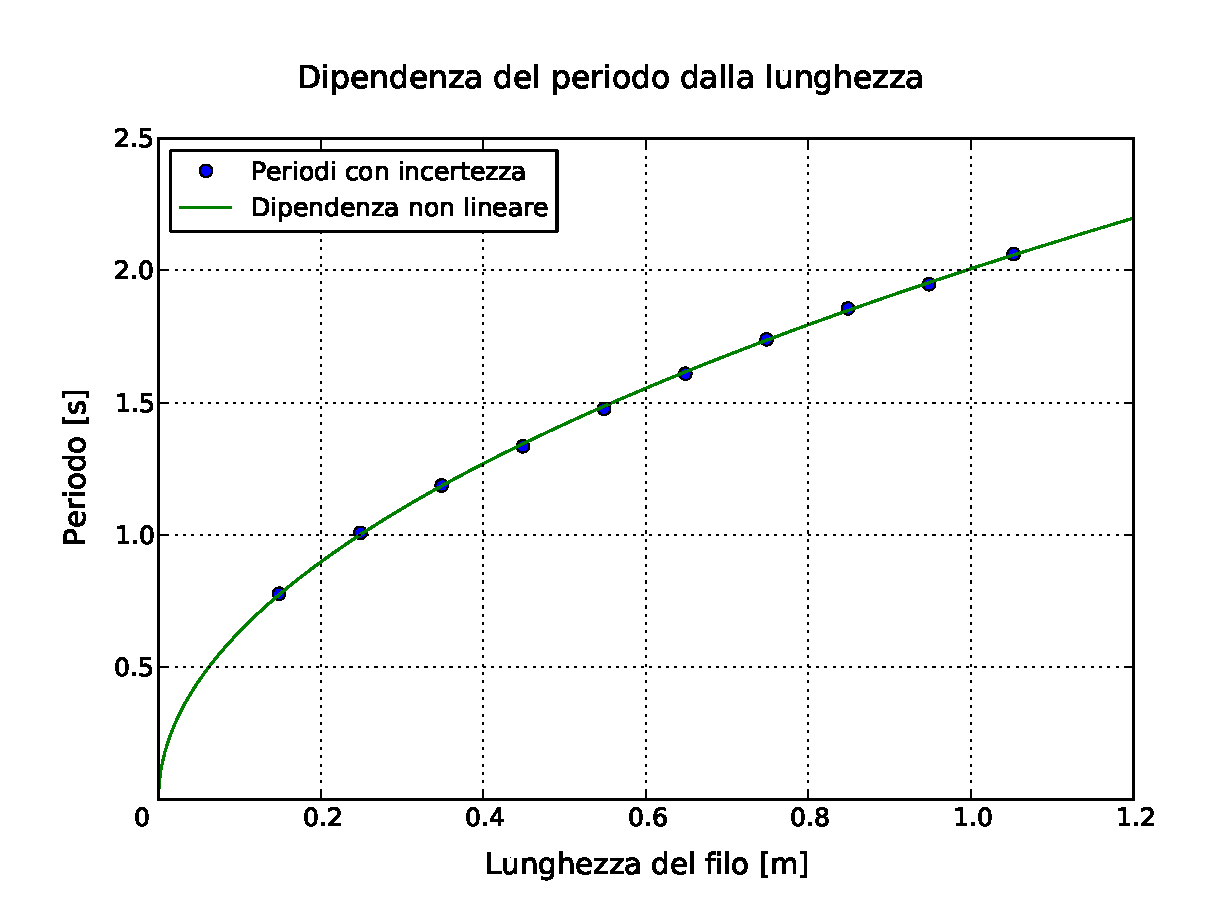
\includegraphics[width=120mm]{immagini/lunghezza_periodo.pdf}
    \caption{}
    \label{fig:lunghezza_periodo}
\end{SCfigure}

\begin{equation}
    \mathcal{T} = 2\pi\sqrt{\frac{\ell}{g}}
    \tag{\ref{eq:periodo_pendolo}}
\end{equation}
%
tuttavia qui assumiamo solo che i punti del grafico seguano una legge del tipo:

\begin{equation}
    \mathcal{T} = a\ell^b
    \label{eq:ipotesi}
\end{equation}
%
dove a e b sono due costanti. Dal grafico si può intuire una dipendenza di questo tipo.
Andremo quindi a verificare la legge (\ref{eq:periodo_pendolo}).
Al fine di linearizzare la (\ref{eq:ipotesi}) per poter utilizzare la regressione, definiamo due nuove variabili:

\begin{equation}
    X := \log_{10}{(\ell)} \qquad \qquad Y := \log_{10}{(\mathcal{T})}
\end{equation}

Le incertezze su $X$ e $Y$, calcolate con le solite regole di propagazione, sono

\begin{equation}
    \delta Y = \frac{\log_{10}(e)}{\mathcal{T}}\delta\mathcal{T}
    \qquad \qquad
    \delta X = \frac{\log_{10}(e)}{\ell}\delta \ell
\end{equation}

Quindi la (\ref{eq:ipotesi}) diventa

\begin{equation}
    Y = \log_{10} a + b \log_{10} \ell = A + b \log_{10} \ell
\end{equation}
%
dove $A := \log_{10} a$ e dunque $a = 10^A$.

%\begin{table}
%    \centering
%    \begin{tabular}{c c c c}
%    \end{tabular}
%\end{table}

Procediamo ora con il calcolo dei parametri A e b tramite regressione lineare. 
La regressione si basa sulla minimizzazione della funzione

\begin{equation}
    \sum_{i=1}^N \frac{(Y_i - A - bX_i)^2}{\delta Y\ped{tot}}
    \label{eq:min_quad}
\end{equation}
%
che misura la discrepanza tra legge lineare e dati sperimentali. Minimizzando la (\ref{eq:min_quad}) si ottengono
i valori di $A$ e $b$, ovvero la retta, che interpretano in modo ``migliore'' i dati.
Come prima cosa stimiamo il parametro b
per trasferire l'incertezza dalle X alle Y. La stima è stata ottenuta ignorando l'incertezza sulle X e facendo un fit preliminare.


\begin{equation}
    A = 0.69631 \qquad \qquad b = 0.49915
\end{equation}

Le incertezze su $A$ e $b$ valgono:

\begin{equation}
    \delta A = 0.0010388 \qquad \qquad \delta b = 0.0018843
\end{equation}

Risaliamo quindi al valore di a:

\begin{equation}
    a = 2.0063 \qquad \qquad \delta a = 0.0039972
\end{equation}
